\begin{tikzpicture}[scale=1,transform shape]
	\draw (0, 0) rectangle (7, 2);
	\draw (3.5,1) node[text width=3.5cm] {Neural network with $L-1$ hidden layers};
	\draw[thick,->] (1,-1) -- (1,0);
	\draw[thick,->] (2,-1) -- (2,0);
	\draw[thick,->] (3,-1) -- (3,0);
	\draw[thick,->] (4,-1) -- (4,0);
	\draw[thick,->] (5,-1) -- (5,0);
	\draw[thick,->] (6,-1) -- (6,0);
	\draw[thick,->] (1.4,2) -- (1.4,3) node[above] {\footnotesize Apple};
	\draw[thick,->] (2.8,2) -- (2.8,3) node[above] {\footnotesize Mango};
	\draw[thick,->] (4.2,2) -- (4.2,3) node[above] {\footnotesize Orange};
	\draw[thick,->] (5.6,2) -- (5.6,3) node[above] {\footnotesize Banana};
	\draw (3.1,3.5) node[above] {\large $y = \left[ 1 \hspace{1.2cm} 0 \hspace{1.2cm} 0 \hspace{1.2cm} 0 \right]$};
	\node[inner sep=0pt] (russell) at (3.5,-2)
	{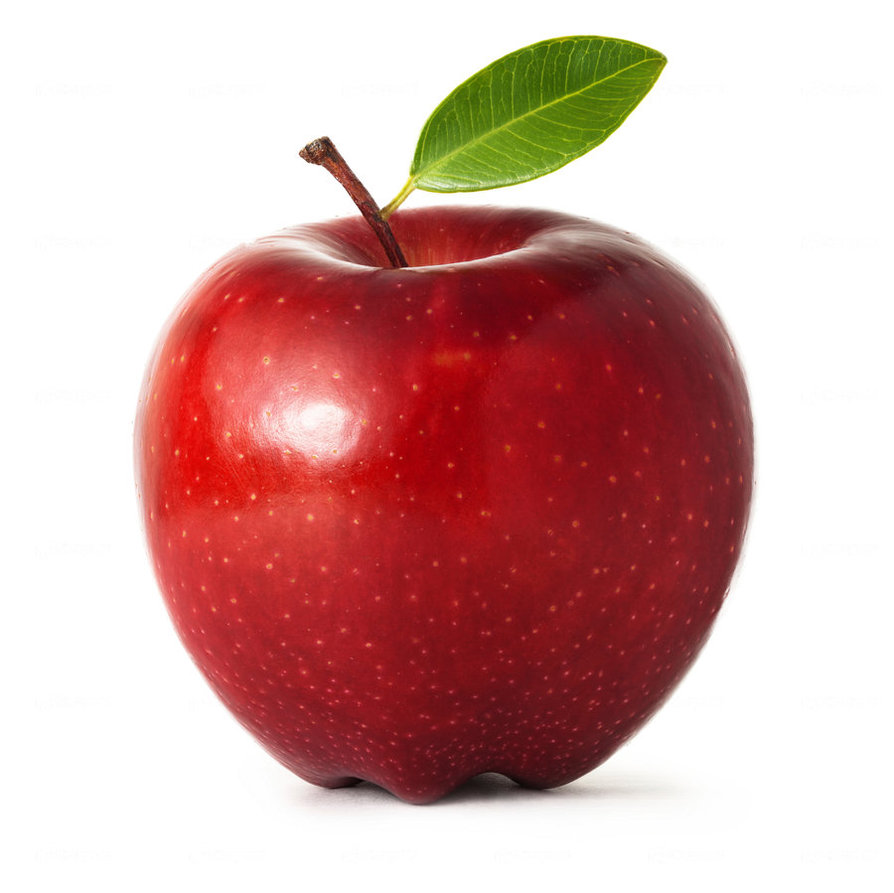
\includegraphics[width=.25\textwidth]{apple.jpg}};
\end{tikzpicture}
